\documentclass{article}
\usepackage[english]{babel}
\usepackage[letterpaper,top=2cm,bottom=2cm,left=3cm,right=3cm,marginparwidth=1.75cm]{geometry}
\usepackage{amsmath}
\usepackage{graphicx}
\usepackage[colorlinks=true, allcolors=blue]{hyperref}
\usepackage[numbers]{natbib}
\usepackage{listings}
\usepackage{subcaption}

\title{NOvA Production 6 Validation Task Force Contribution Summary}
\author{Jiaxi Liu}

\begin{document}
\maketitle

\section{Task Description}

The purpose of this study is to validate the TransformerCVN~\cite{TransformerCVN}
 model by checking whether its results are reasonable and consistent with existing models (EventCVN \& ProngCVN) and data. The validation consists of three parts. The first two parts are complete:

\paragraph{Data / MC Comparison (ND only)} 
We compare data with Monte Carlo simulation for the Near Detector to check for any significant discrepancies in the TransformerCVN predictions. Event-level and prong-level score distributions are examined as a function of energy for each output category. Consistent PID distributions are observed for all major event classes, with no significant shape discrepancies~\cite{docdb-69340}.

\paragraph{MC-to-MC Comparison (ND and FD)} 
We compare Prod5.1 (which uses EventCVN for event-level classification and ProngCVN for prong-level classification) against Prod6 (which introduces TransformerCVN for both tasks) using Monte Carlo simulations for both the Near and Far Detectors, across all four beam configurations: FD FHC, FD RHC, ND FHC, and ND RHC. The validation covers event-level and prong-level score distributions, confusion matrices, and ROC curves. The full validation results can be found here~\cite{docdb-70060}.


At event-level, no discrepancies are found between the two models. At prong-level, poor electron performance is observed for $\nu_e$-CC events due to a truth labeling issue: During model training, the true labels used are no longer stored in the official dataset, making it impossible to use exactly the same truth labels for validation.~\cite{docdb-69385} This discrepancy has the largest impact on the electron category. After applying strict cuts on prong efficiency/purity to remove most of the mislabeled electrons, the final trend is finally consistent with the results previously seen when training on MiniProd6.1OPAL samples. For $\nu_\mu$-CC events, We also observed a discrepancy between TransformerCVN and ProngCVN in pion identification performance, with TransformerCVN appearing worse, as shown in Figure~\ref{fig:jliu-cm-prong}. However, after using the primary particle list for validation to avoid the impact of the truth labeling issue, the final results show that TransformerCVN matches or even exceeds ProngCVN in pion identification~\cite{docdb-70060}, see Figure~\ref{fig:jliu-pionid-auc}.

\paragraph{Threshold for Acceptance} 
The remaining work includes verifying that the performance of TransformerCVN is equivalent to or better than what was seen in MiniProd6.1, and checking the consistency of PID scores across data and MC. 




\begin{figure}[t]
    \centering
    \IfFileExists{images-jliu/cm_4class_fd_fhc_eff.png}{%
        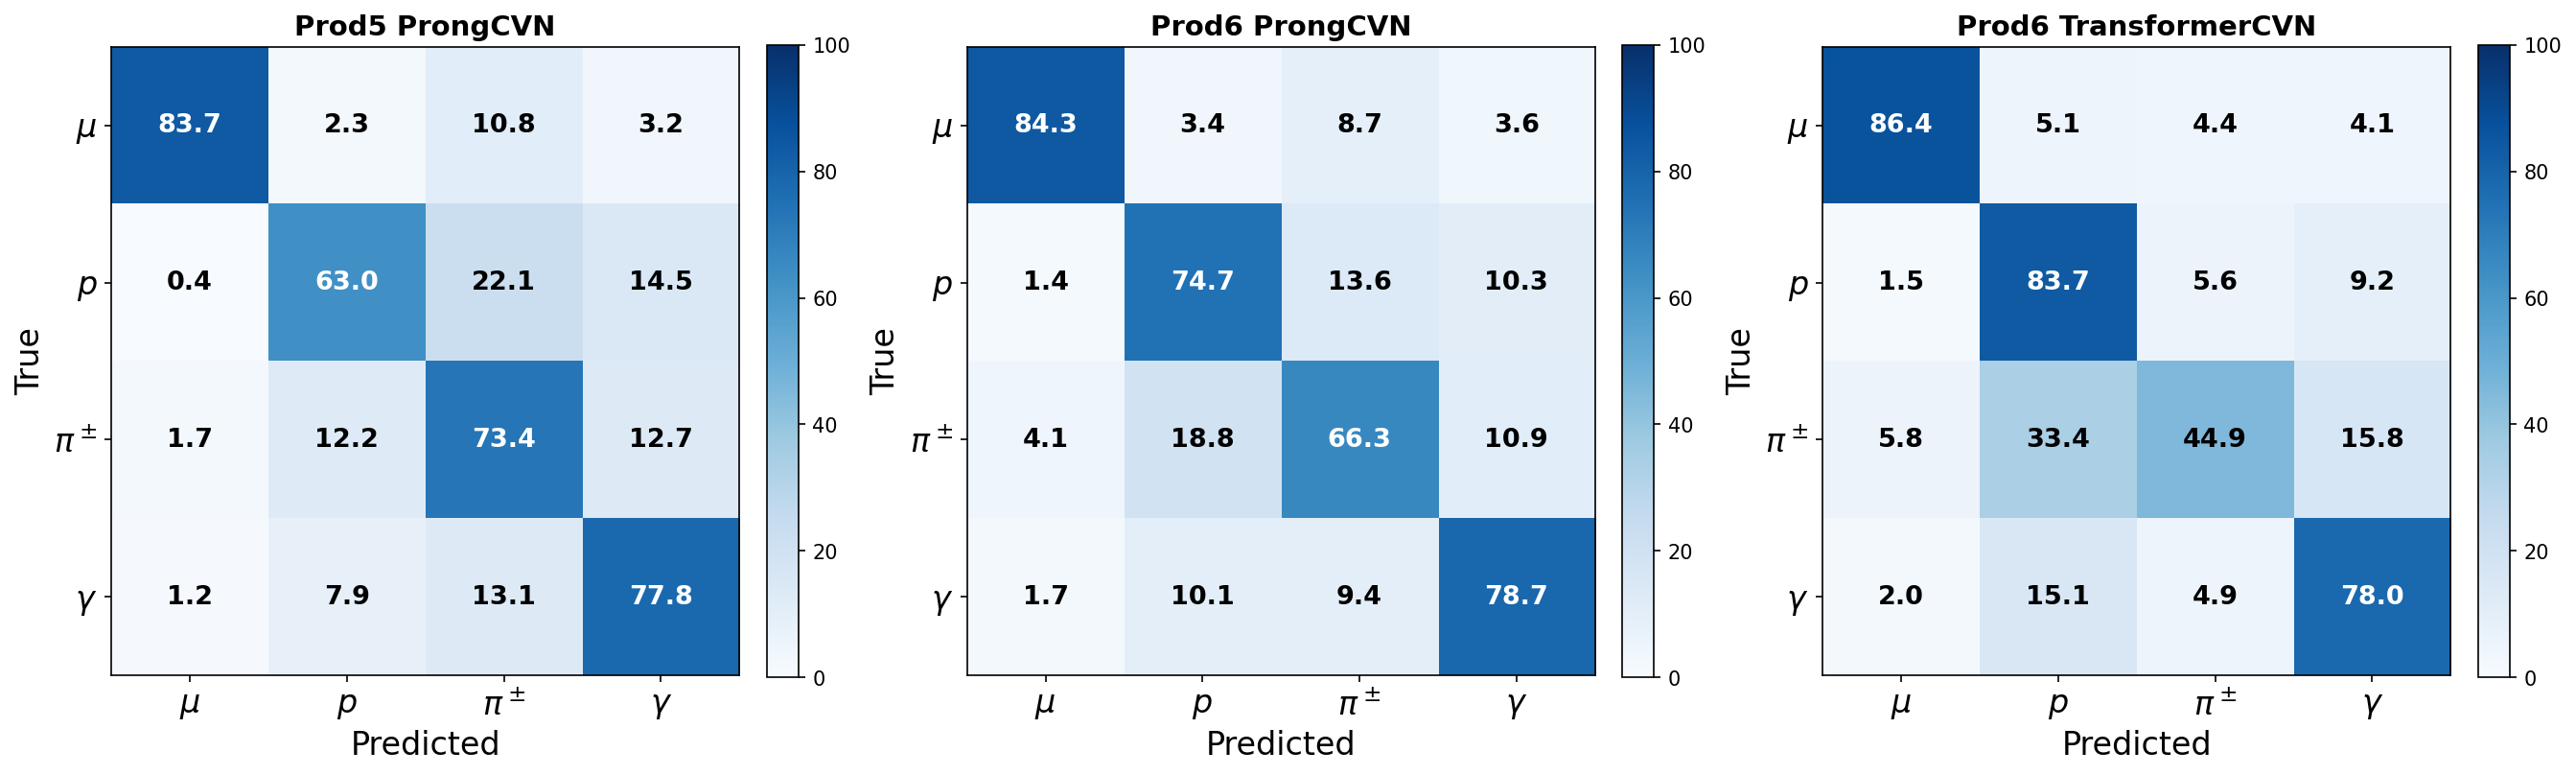
\includegraphics[width=0.75\textwidth]{images-jliu/cm_4class_fd_fhc_eff.png}%
    }{\fbox{\parbox[c][0.12\textheight][c]{0.95\textwidth}{\centering Efficiency}}}
    \vspace{2pt}
    \IfFileExists{images-jliu/cm_4class_fd_fhc_pur.png}{%
        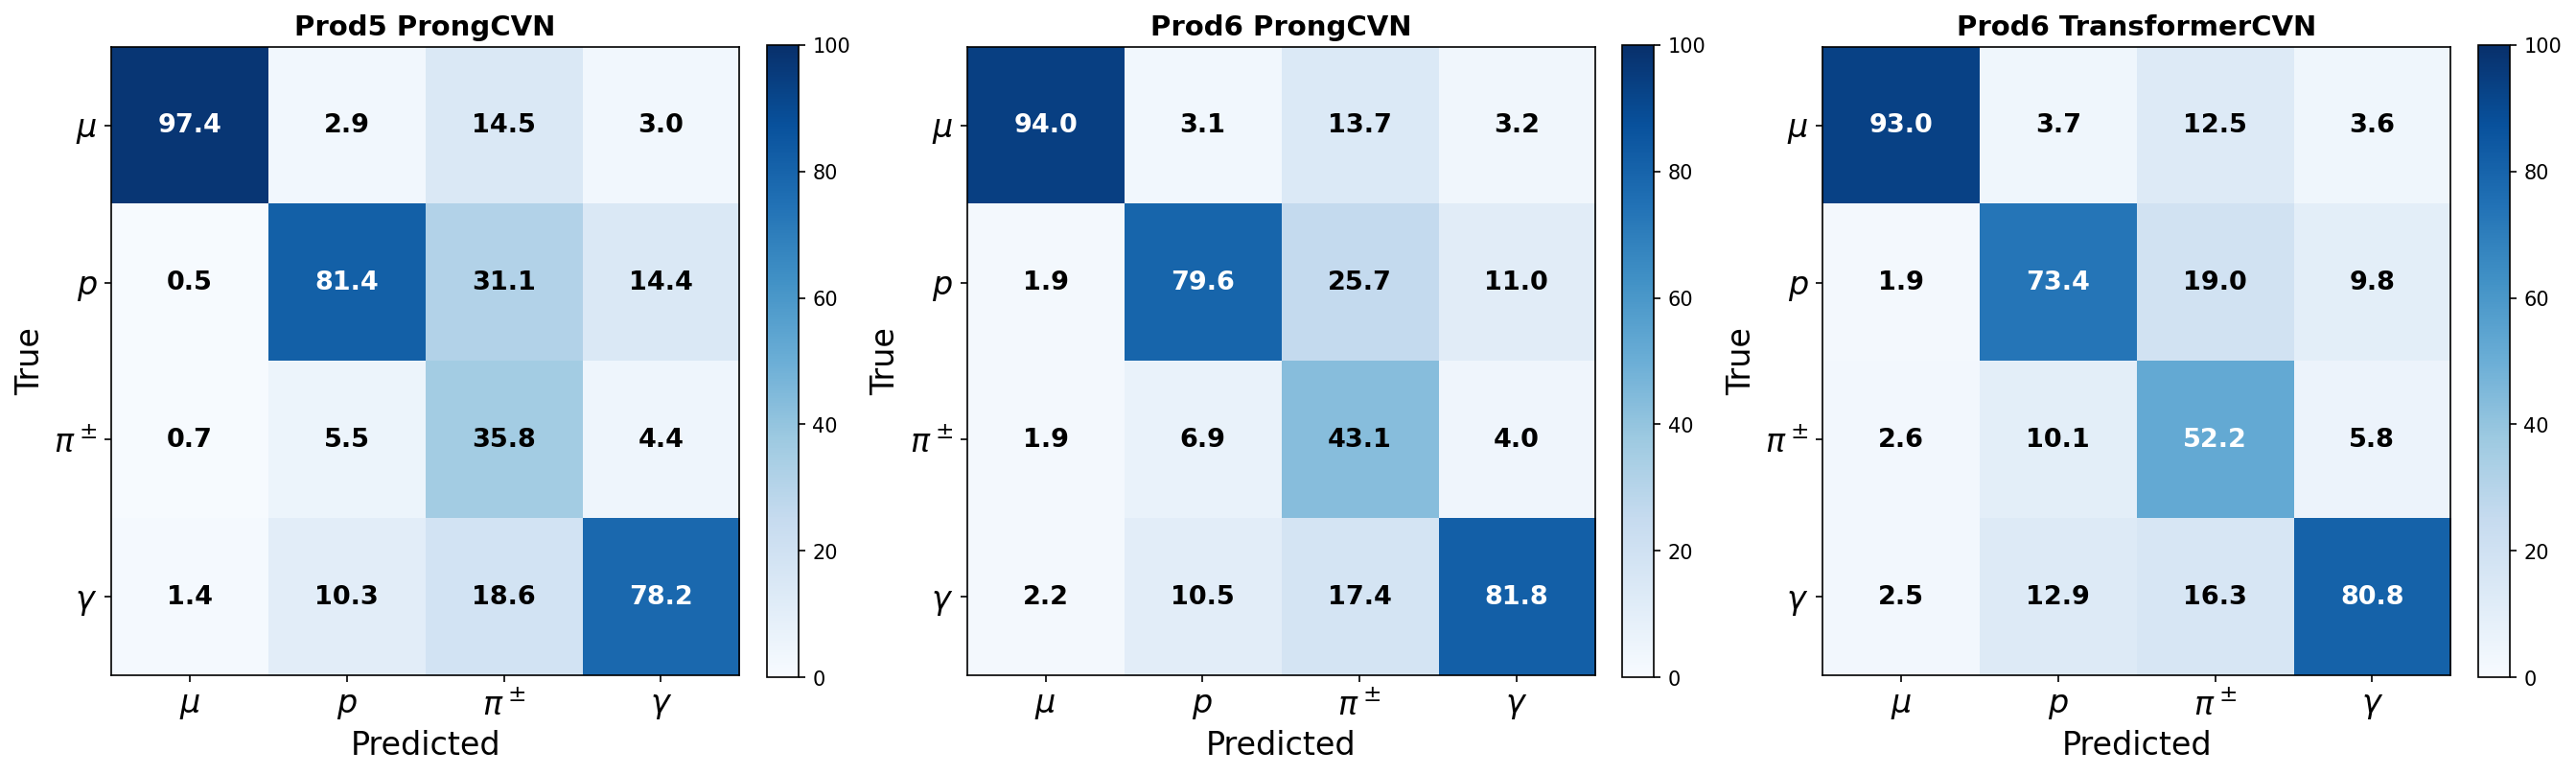
\includegraphics[width=0.75\textwidth]{images-jliu/cm_4class_fd_fhc_pur.png}%
    }{\fbox{\parbox[c][0.12\textheight][c]{0.95\textwidth}{\centering Purity}}}
    \caption{Prong-level 4-class confusion matrices for $\nu_\mu$-CC events in FD FHC, comparing Prod5.1 ProngCVN, Prod6 ProngCVN, and Prod6 TransformerCVN. Top: efficiency; bottom: purity.}
    \label{fig:jliu-cm-prong}
\end{figure}

\begin{figure}[t]
    \centering
    \IfFileExists{images-jliu/pionid_auc_summary.png}{%
        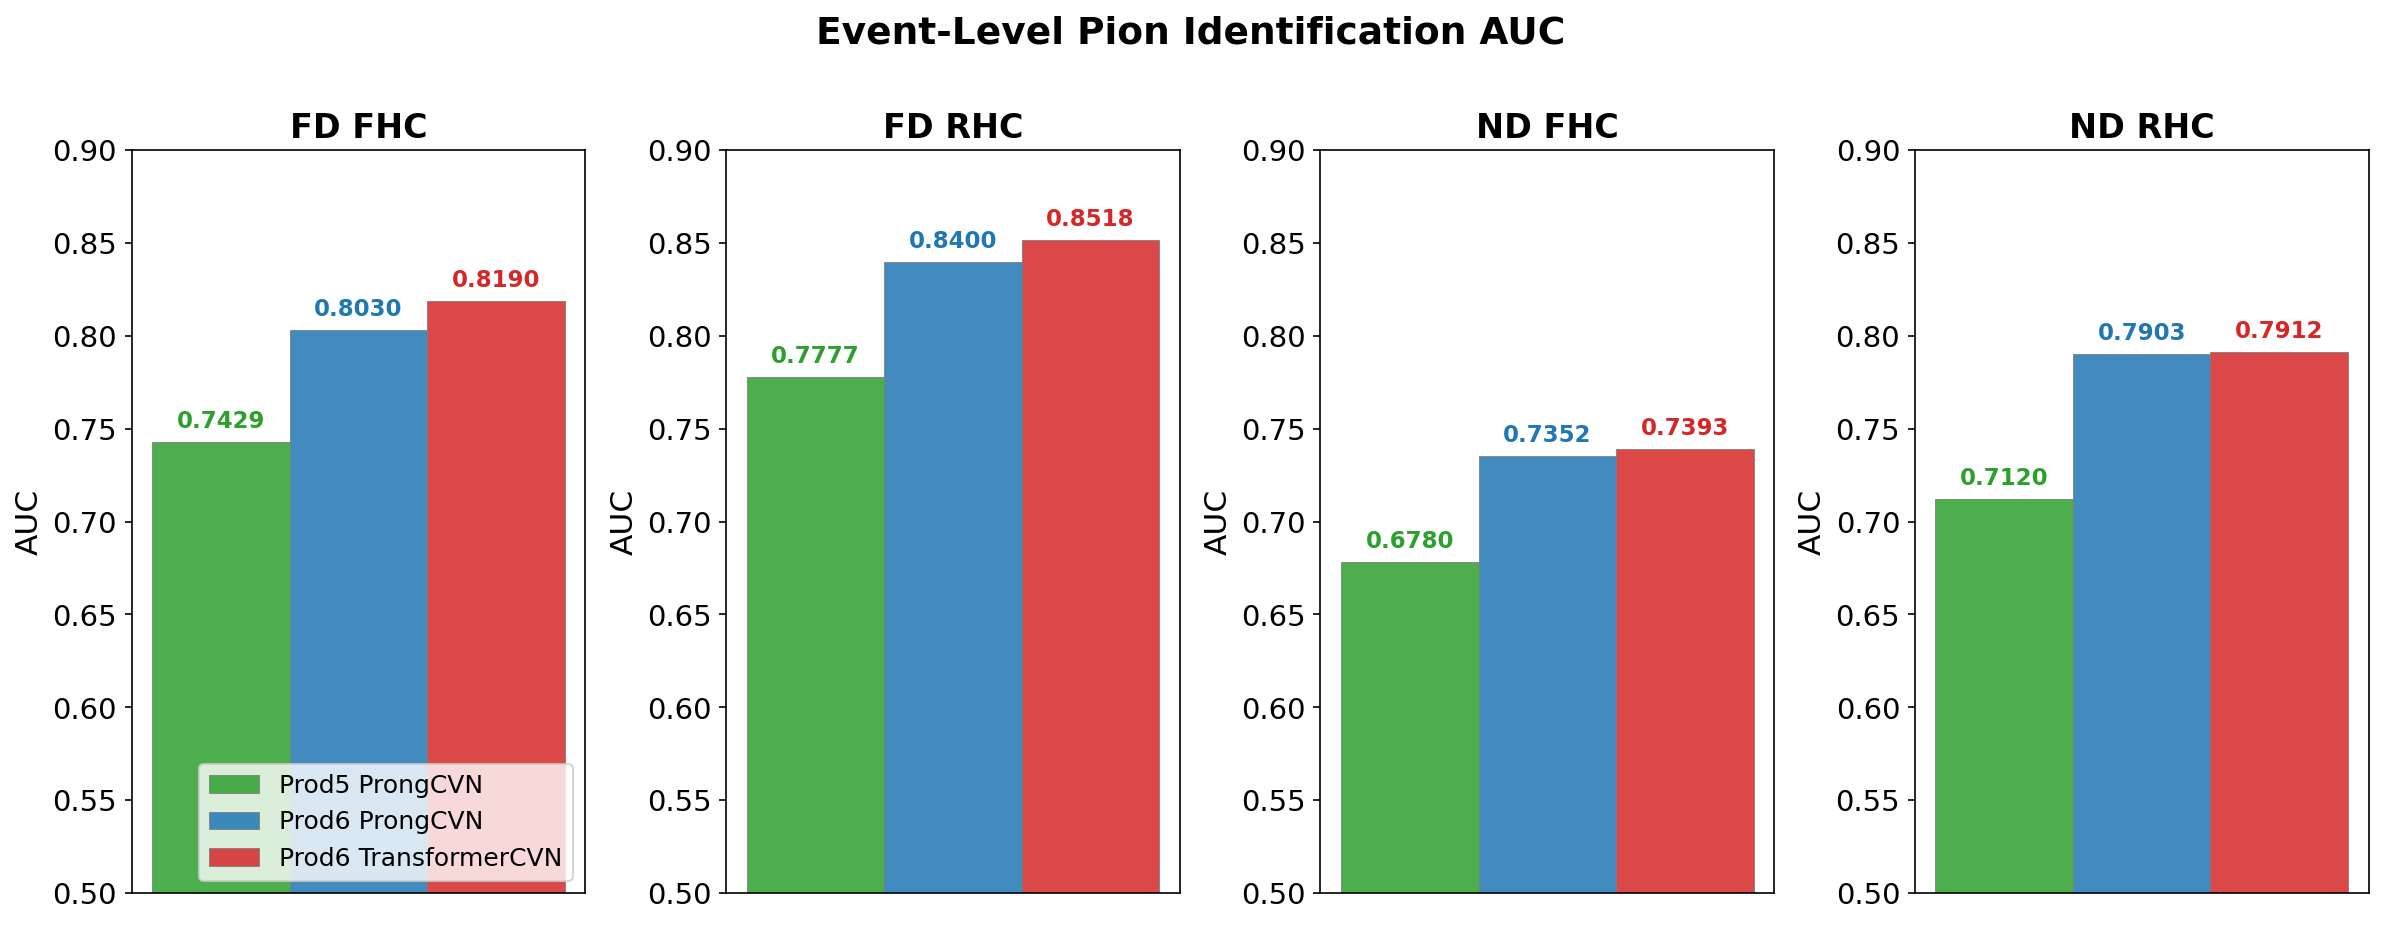
\includegraphics[width=0.85\textwidth]{images-jliu/pionid_auc_summary.png}%
    }{\fbox{\parbox[c][0.15\textheight][c]{0.95\textwidth}{\centering PionID AUC}}}
    \caption{Event-level pion identification AUC for $\nu_\mu$-CC events with exactly one muon and at least one pion in the primary particle list, comparing Prod5.1 ProngCVN, Prod6 ProngCVN, and Prod6 TransformerCVN across all four beam configurations. AUC values are computed from the ROC curves of the highest pion score among all prongs versus a background of other primary particle types.}
    \label{fig:jliu-pionid-auc}
\end{figure}

\section{A Complete List of Relevant Docdbs with Citations Including URL}

\bibliographystyle{unsrtnat}
\bibliography{summary-jliu}
\end{document}
